\documentclass[a4paper, 12pt]{article}%тип документа

%отступы
\usepackage[left=1.5cm,right=1cm,top=2cm,bottom=3cm,bindingoffset=0cm]{geometry}
\setlength{\parindent}{5ex}

%Русский язык
\usepackage[T2A]{fontenc} %кодировка
\usepackage[utf8]{inputenc} %кодировка исходного кода
\usepackage[english,russian]{babel} %локализация и переносы

%Вставка картинок
\usepackage{graphicx}
\graphicspath{{pictures/}}
\DeclareGraphicsExtensions{.pdf,.png,.jpg,}
\usepackage{wrapfig}

%Графики
\usepackage{pgfplots}
\pgfplotsset{compat=1.9}

%Математика
\usepackage{amsmath, amsfonts, amssymb, amsthm, mathtools}

%Таблицы
\usepackage{longtable} 
\usepackage{float}

%Римские цифры
\newcommand{\RomanNumeralCaps}[1]{\uppercase\expandafter{\romannumeral#1}}

\usepackage{multirow}



\begin{document}
	\begin{titlepage}
		\begin{center}
			\textsc{Федеральное государственное автономное образовательное учреждение высшего образования«Московский физико-технический институт (национальный исследовательский университет)»\\[5mm]
			}
			
			\vfill
			
			\textbf{Отчёт по лабораторной работе 5.8.1\\[3mm]
				Тепловое излучение
				\\[50mm]
			}
			
		\end{center}
		
		\hfill
		\begin{minipage}{.5\textwidth}
			Выполнил студент:\\[2mm]
			Сериков Василий Романович\\[2mm]
			группа: Б03-102\\[5mm]
			
		\end{minipage}
		\vfill
		\begin{center}
			Москва, 2023 г.
		\end{center}
		
	\end{titlepage}
	
	\newpage
	\setcounter{page}{2}
	\textbf{Аннотация}\\
	
	\textbf{Цель работы: }\\
	
	При помощи модели абсолютно чёрного тела проведение измерения температуры оптическим пирометром с исчезающей нитью и термопарой. Исследование излучение накалённых тел с различной испускательной способностью. Определение постоянных Планка и Стефана-Больцмана
	
	\textbf{Теория: }\\
	
	Для измерения температуры разогретых тел, удалённых от наблюдателя, применяют методы оптической пирометрии, основанные на использовании зависимости испускательной способности исследуемого тела от температуры. Различают три температуры, функционально связанные с истинной термодинамической температурой и излучательной способностью тела: радиационную $T_{rad}$, цветовую $T_{col}$ и яркостную $T_{br}$. \par
	В работе измеряется яркостная температура. Яркостная температура - это температура абсолютно чёрного тела, при которой его спектральная испускательная способность равна спектральной испускательной способности исследуемого тела при той же длине волны.
	Измерение яркостной температуры раскалённого тела производится при помощи оптического пирометра с исчезающей нитью, основанного на визуальном сравнении яркости раскалённой нити с яркостью изображения исследуемого тела. \par
	Яркостная температура тела всегда ниже его термодинамической температуры. Это связано с тем, что любое нечёрное тело излучает меньше, чем АЧТ при той же температуре. Зависимость между яркостной и термодинамической температурами вольфрама приведена на рис. 1
	
	\begin{figure}[H]
		\centering
		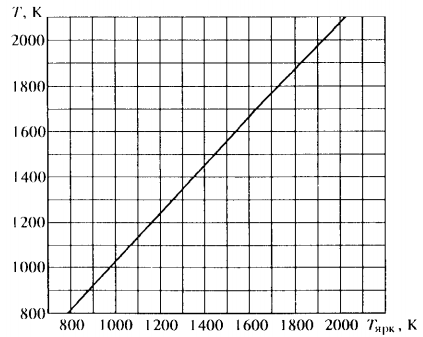
\includegraphics[width=10cm]{fig2}
		\caption{График зависимости $T = f(T_{br})$ для вольфрама}
	\end{figure}
	
	По результатам измерений мощности излучения вольфрамовой нити можно судить о справедливости закона Стефана-Больцмана. Если бы нить излучала как АЧТ, то баланс потребляемой и излучаемой энергии определялся бы соотношением 
	\begin{equation}
		W = \sigma S (T^4 - T_0^4),
	\end{equation}
	где $W$ - потребляемая нитью электрическая мощность, $S$ - площадь излучающей поверхности нити, $T$ - температура нити, $T_0$ - температура окружающей среды. Однако вольфрамовая нить излучает как серое тел, и излучение её ослаблено по сравнению с АЧТ в $\varepsilon_T$ раз для любой волны при данной температуре тела Т. Тогда предположив, что нить излучает как серое тело и с учётом того, что $T_0 \ll T$, выражение (1) можно переписать в виде
	\begin{equation}
		W = \varepsilon_T S \sigma T^4
	\end{equation}
	%В справедливости закона Стефана-Больцмана можно убедиться, построив график зависимости $W(T)$ в логарифмическом масштабе и по углу наклона определить показатель степени $n$ исследуемой температурной зависимости. В пределах погрешности показатель степени должен быть близок к четырём. \par%
	
	\textbf{Экспериментальная установка: }\\
	
	\begin{figure}[h]
		\centering
		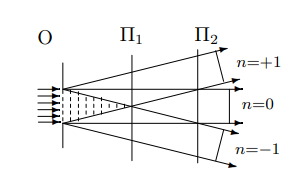
\includegraphics[width=11cm]{fig1.PNG}
		\caption{Схема экспериментальной установки: 1 - блок питания; 2 - тумблер включения питания образцов; 3 - тумблер нагрева нити пирометра; 4 - кнопка "Нагрев нити"; 5 - кнопка "охлаждение нити"; 6 - тумблер переключения образцов; 7 - регулятор мощности нагрева образцов; 8 - окуляр пирометра; 9 - корпус пирометра; 10 - объектив пирометра; 11 - переключение диапазонов; 12 - ручка смещения красного светофильтра; 13 - регулировочный винт; 14 - вольтметр (напряжение на лампе накаливания); 15 - амперметр (ток через образцы); 16 - вольтметр в цепи термопары; 17 - модель АЧТ; 18 трубка с кольцами из материалов с различной излучательной способностью; 19 - лампа накаливания; 20 - неоновая лампочка}
		\label{fig:vac}
	\end{figure}
	
		Используемые образцы - керамическая трубка, закрытая с одного конца и окружённая для теплоизоляции внешним кожухом. Температура в трубке измеряется с помощью термопары хромель-алюмель, керамическая трубка с набором колец из различных материалов, нагреваемая изнутри нихромовой спиралью. Материалы колец имеют различную излучательную способность и вольфрамовая нить электрической лампочки.\\
	
	\newpage
	
	\textbf{Ход работы: }\\
	
	\begin{enumerate}
		
		\item Проведем сравнение показаний температуры АЧТ пирометра и термопары. Снимем несколько значений температуры с пирометра и напряжения на термопаре. По графику зависимости температуры от напряжения (рис3.) на термопаре определим температуру АЧТ 
		
		\begin{figure}[H]
			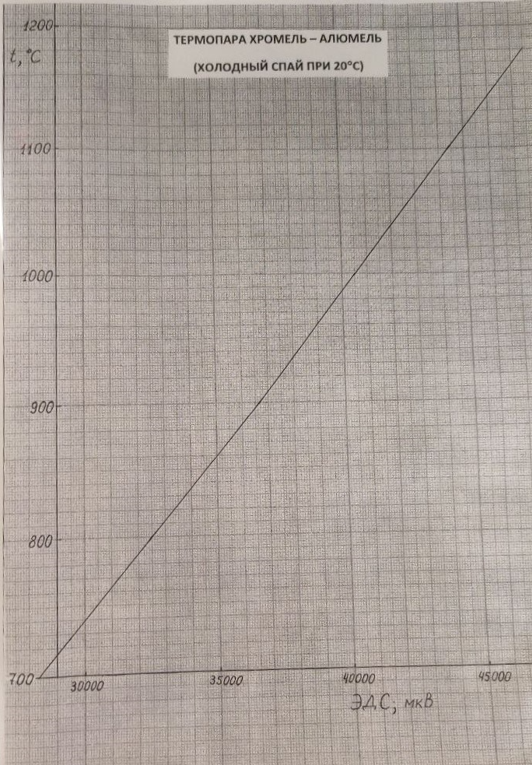
\includegraphics[scale=0.9]{t(U)}
			\centering
			\caption{График зависимости $t(U)$}
		\end{figure}
		
		
		\begin{longtable}{|c|c|c|c|c|c|}
			\hline
			№ & 1 & 2 & 3 & 4 & 5\\ \hline
			$U, $ мВ & 36,7 & 37,5 & 38,1 & 38,7 & 39,5 \\ \hline
			$t_{\text{термопара}}$, $^\circ C$ & 900 & 922 & 937 & 956 & 970 \\ \hline
			$t_{\text{пирометр}}$, $^\circ C$ & 881 & 902 & 915 & 960 & 980 \\ \hline
			\caption{Полученные двумя способами данные температуры АЧТ, $\sigma_U = 0,1$ мВ, $\varepsilon_{t_{\text{термопара}}} = \varepsilon_U$, $\varepsilon_{t_{\text{пирометр}}} = 1\%$}
		\end{longtable}
		
		
		\newpage
		
		\item Проведем измерение яркостной температуры керамической трубки с двумя кольцами из разных материалов. Полученные измерения занесем в таблицу 2.
		
		\begin{longtable}{|c|c|c|}
			\hline
			$t_{\text{трубка}}, ^\circ C$ & $t_{\text{кольцо}1}, ^\circ C$ &  $t_{\text{кольцо}2}, ^\circ C$ \\ \hline
			940 $\pm$ 10 & 820 $\pm$ 10 & 889 $\pm$ 10 \\ \hline
			\caption{Температуры керамической трубки и двух колец, определенные с помощью пирометра}
		\end{longtable}
		
		
		\item Проведем проверку закона Стефана-Больцмана. Для этого постепенно будем увеличивать накал нити накаливания лампы и снимать показания пирометра, напряжение и ток через нить. Переведем яркостную температуру в термодинамическую по графику, изображенному на Рис1. Результаты запишем в таблицу 3. По полученным данным построим график зависимости $\ln W = \ln(\varepsilon_T B) + n\ln T$, где $W$ -- мощность, $\varepsilon_T$ находится из таблицы на Рис4, $B = \sigma \cdot S$, S = 5 см$^2$, $\sigma$ -- постоянная Стефана-Больцмана. 
		
 
		\begin{longtable}{|c|c|c|c|c|}
			\hline
			№ & $U,$ В & $I,$ А & $t_{\text{ярк.}},$ $ ^\circ C$ & $t_{\text{терм.}},$ К\\ \hline
			1 & 27,7 & 0,73 & 930 & 1203 \\\hline
			2 & 38,1 & 0,85 & 1130 & 1403 \\\hline
			3 & 45,4 & 0,92 & 1200 & 1473\\\hline
			4 & 58,9 & 1,06 & 1360 & 1633\\\hline
			5 & 70,1 & 1,16 & 1500 & 1773\\\hline
			6 & 70,1 & 1,24 & 1650 & 1923\\\hline
			7 & 87,7 & 1,31 & 1760 & 2033\\\hline
			8 & 92,0 & 1,34 & 1900 & 2173\\\hline
			9 & 106,3 & 1,45 & 2010 & 2283\\\hline
			10 & 117,9 & 1,53 & 2100 & 2373\\\hline
			\caption{Значения напряжения, тока, температуры для нити накаливания $\sigma_U = 0,1$ В, $\sigma_I = 0,01$ А, $\varepsilon_{t_{\text{ярк.}}} = \varepsilon_{t_{\text{терм.}}} = 1\%$}
		\end{longtable}
		
		\begin{figure}[H]
			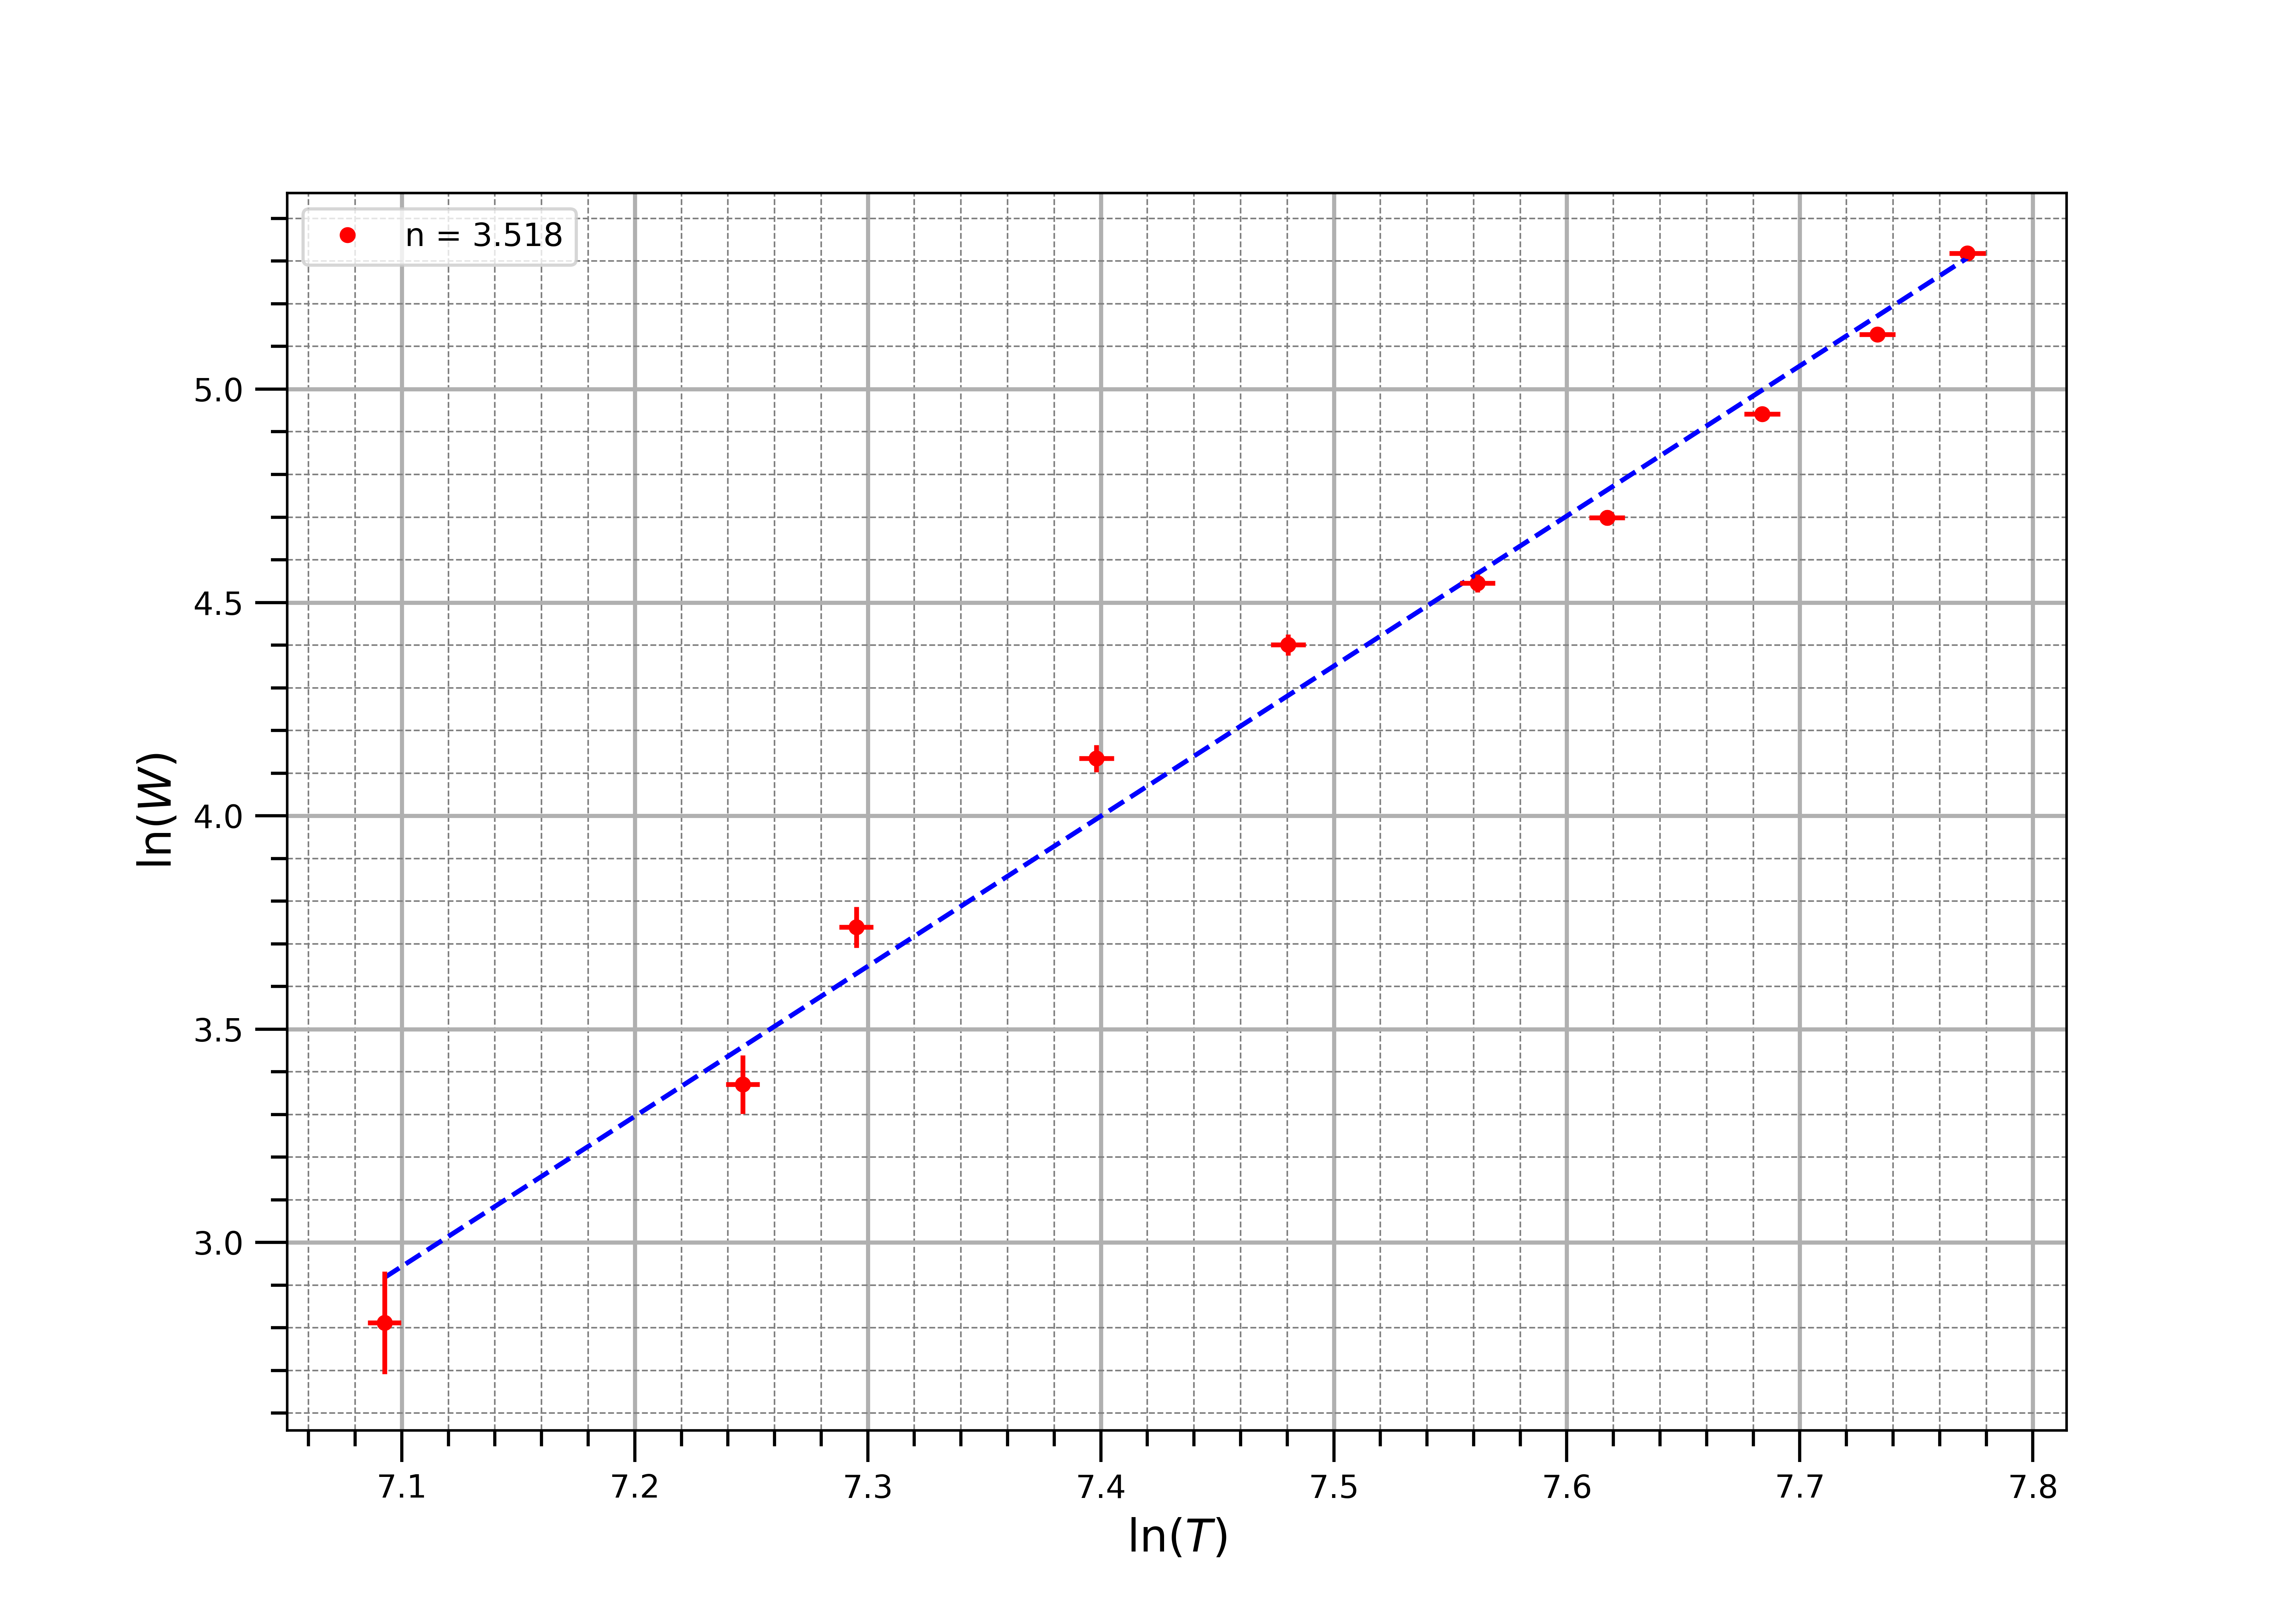
\includegraphics[scale=0.8]{W}
			\centering
			\caption{График зависимости $\ln W = \ln(\varepsilon_T B) + n\ln T$}
		\end{figure}
		
		\begin{figure}[H]
			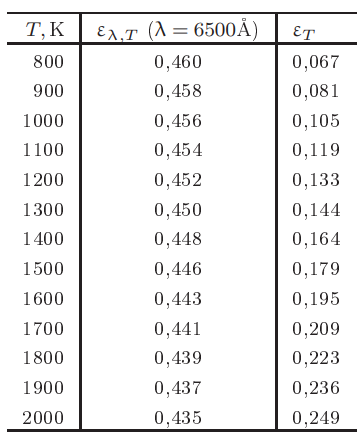
\includegraphics[scale=0.9]{eps}
			\centering
			\caption{Поправочные коэффициенты излучения для вольфрама}
		\end{figure}
		
		
		\item Для температур выше 1700 $^\circ$K определим $\sigma$ по формуле:
		
		$$ W = \varepsilon_T S \sigma T^4 $$
		
		\item По найденным $\sigma$ определим величину постоянной Планка по формуле: 
		
		$$ h = \sqrt[3]{\frac{2\pi^5k_{\text{б}}^4}{15c^2\sigma}} $$
		
		\begin{longtable}{|c|c|c|c|c|c|c|}
			\hline
			T, К & 2373 & 2283 & 2173 & 2033 & 1923 & 1773 \\\hline
			  $h$, Дж$\cdot$ с $\cdot 10^{-34}$& 3,40 & 3,45 & 3,44 & 3,42 & 3,34 & 3,15 \\ \hline
			$\sigma$, Вт$\cdot$cм$^{-2} \cdot K^{-4}$ $\cdot 10^{-11}$ & 4,15 & 3,99 & 4,02 & 4,10 & 4,37 & 5,21 \\ \hline
			\caption{Рассчитанные значения $\sigma$ и $h$.  $\varepsilon_T = 1\%$ В, $\varepsilon_{\sigma} \approx 4\varepsilon_T = 4\%$, $\varepsilon_{h} \approx 1/3\varepsilon_{\sigma} = 1,3\%$}
		\end{longtable}
		
		
		$$ \overline{h} = (3,38 \pm 0,04)\cdot 10^{-34} \text{Дж с}$$
		
		$$ \overline{\sigma} = (4,2 pm 0,1) \cdot 10^{-11} \text{Вт}\cdot \text{см}^{-2} \cdot K^{-4} $$
		
		
		\textbf{Обсуждение результатов и выводы: }\\
		
		В ходе данной работы мы познакомились с понятием яркостная температура. Изучили модель абсолютно черного тела, исследовали излучение накаленных тел с различной испускательной способностью. Определили постоянную Планка  $ \overline{h} = (3,38 \pm 0,04)\cdot 10^{-34} \text{Дж с}$, которая по порядку величины совпадают с табличным значением: 6,63 $\cdot$ 10$^{-34}$ Дж с. Также определили постоянную Стефана-Больцмана $ \overline{\sigma} = (4,2 \pm 0,1) \cdot 10^{-11} \text{Вт}\cdot \text{см}^{-2} \cdot K^{-4} $, которая на один порядок отличается от табличного значения $\sigma = 5,67\cdot 10^{-12} \text{Вт}\cdot \text{см}^{-2} \cdot K^{-4} $ 
		
		Основной вклад в ошибку полученных величин вносит погрешность измерения яркостной температуры, так как от способности экспериментатора различать оттенки красного зависит точность экспериментальных данных.
		
		
		
		
		
		
		
		
		
		
		
		
		
		
		
		
		
		
		
		
		
		
		
		
	\end{enumerate}
	
	
	
	
	
	
	
	
	
	
	
	
	
	
	
	
	
	
	
	
	
	
	
	\end{document}